\newcount\Comments  
\Comments=1   
\documentclass[a4paper,12pt, english]{article}
\usepackage[top=2cm, bottom=2cm, left=2cm, right=2cm]{geometry}

\usepackage{babel}
\usepackage{float}
\usepackage{listings}

\usepackage{color}

\definecolor{darkgreen}{rgb}{0,0.5,0}
\definecolor{purple}{rgb}{1,0,1}
%\usepackage{subcaption}

\newcommand{\kibitz}[2]{\ifnum\Comments=1\textcolor{#1}{#2}\fi}
% add yourself here:
\newcommand{\ls}[1]{\kibitz{red}      {[Larisa: #1]}}
\newcommand{\cg}[1]  {\kibitz{purple}   {[Crina: #1]}}
\newcommand{\ns}[1]{\kibitz{cyan}     {[Noureddin: #1]}}


\usepackage{graphicx}
\usepackage{caption}

\usepackage{listings}
\usepackage{url}


\usepackage{subcaption}
\usepackage{subfig}
\usepackage{verbatim}

\usepackage{array}
\usepackage{booktabs}
\setlength{\heavyrulewidth}{1.5pt}
\setlength{\abovetopsep}{4pt}

%\usepackage{caption}
%\usepackage{enumitem}

%\onehalfspacing

\begin{document}

\title{Regression Analysis}
%\date{Mar 2014}
%\author{By: Noureddin Sadawi}
\maketitle

\section{Introduction}
Regression analysis is a powerful technique that can be used to address various research questions. In this report, we are going to use it to check how q levels are affected by cu and phi. In particular, the type of regression we are going to use is "Multiple Linear Regression". Linear regression is the process of finding the best-fitting straight line through data points (this line is sometimes referred to as the regression line). Multiple means we have more than one input variable (also known as predictor), hence, we are trying to fit a plane or hyper-plane rather than a line.  The input variables in our case are cu, phi and as. Linear means that we are trying to find a combination of the input variables such that each variable is multiplied by a coefficient and then we sum the products. The idea is to use this linear combination of input variables to model their relationship with an output variable (in our case, this is q).

\section{The Modelling Tool}
In order to fit models, we are going to use R~\cite{R} which is a powerful and easy to use tool for statistical computing and graphics. R makes it easy to manipulate data and perform calculations as well as display information graphically. It also facilitates modelling (linear and nonlinear) and other statistical processes.

%\section{Plotting the Data}

\section{The Research Question}
Before we emark on any analysis, let us be clear about what we are addressing.\\
In this report, we will be addressing whether there is any association between VARIABLE(s) and Q.

\section{Diagnostics for Examining a Fit}\label{sec:examine-fit}
There are several diagnostics that can be used to explore the goodness of fit of a model. In the remainder of this report (Section~\ref{sec:checkmodelfit}) we are going to use the following:
\subsection{R-squared}\label{sec:r2}
This value calculates the percentage of variation of the output explained by the input variables in the model. This means the higher the value of R-squared the better the model. 
\subsection{R-squared adjusted}\label{sec:adj-r2}
This value is similar to R-squared but it accounts for the number of input variables in the model, hence, it is sometimes preferred to R-squared.
\subsection{Residuals}\label{sec:residuals}
A residual is the difference between the actual value and predicted value for each point (or record) in the data. Histograms are often used to check the distribution of residuals. Also, they are plotted against each input variable. If a model fits well, the residuals will be small and will be no pattern of their distrbution around zero (i.e. they should be evenly spread around zero).
\subsection{Deviance}\label{sec:dev}
The deviance is a statistic that is used to determine the quality of fit for a model. It is a measure of how much better a model with more parameters fits the data. It is used to compare nested models. A nested model is a model which is a subset of another model. For example, if we have two models, the first describes the relationship between one input variable x and an output variable y and the second describes the relationship between two input variables x and z and an output variable y, then the frist model is nested within the second.

\subsection{Bayesian Information Criterion (BIC)}\label{sec:bic}
When there is a limited number of models, the BIC is often used for model selection. Often, the model with the smallest BIC is preferred. The BIC is a penalised version of the deviance where the penalty is relevant to the number of input variables.

\begin{comment}
\section{Fitting the Models}
Let us begin fitting and examining the models. In the following subsections, we are going to fit all possible combinations of our three input variables.
\subsection{cu vs q} 
In this section, we are going to build a simple linear regression model using just cu as input and q as output. After using R's lm() function, the model looks as follows:\\
\begin{equation}
\label{eq:cu}
q = 92.890    +    8.557*cu 
\end{equation}       
By examining equation~\ref{eq:cu}, we observe that an increase, of decrease, of cu by one unit, causes an increase, or decrease, in q by 8.557 units
\begin{figure}[h!]
  \centering
  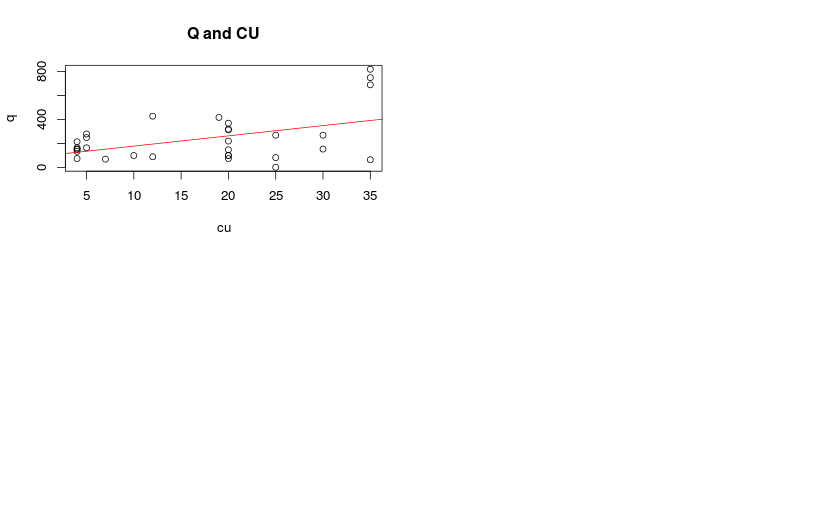
\includegraphics[width=0.6\textwidth]{cu-line}
  \caption{A gull}
  \label{fig:cu-line}
\end{figure}

Let us examine Figure~\ref{fig:cu-goodness}. The top-left plot shows a standard residual plot displaying residuals against fitted values. The labelled points are considered to be outliers. We do not observe any apparent pattern in the points on this plot. The top-right plot is a Q-Q plot of standardized residuals. As we can observe, the errors are approximately normally distributed. The bottom-left plot is a Scale-Location which is the same as standard residual plot (both show no trend to the residuals). The bottom-right plot shows residuals vs. leverage. Any labeled points on this plot should be investigated as they can possibly be having undue influence on the regression relationship.\\
Points 17,23,25 REMOVE?


\begin{figure}[H]
  \centering
  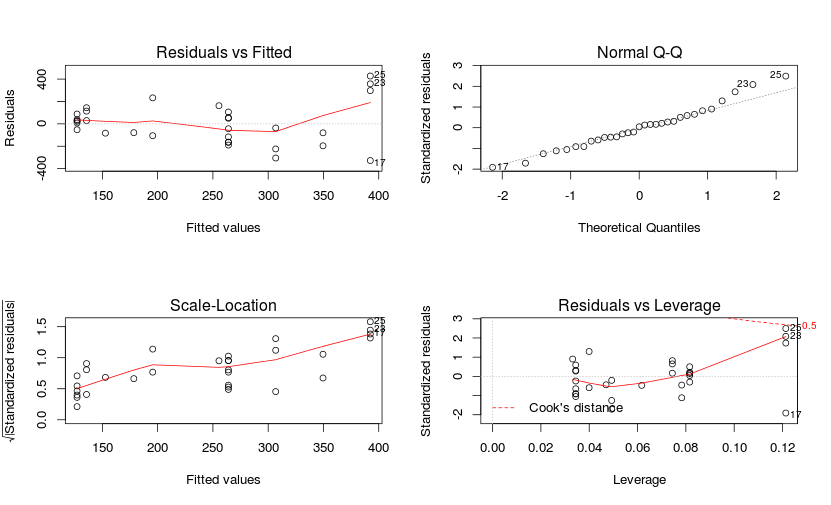
\includegraphics[width=0.6\textwidth]{cu-goodness}
  \caption{A gull}
  \label{fig:cu-goodness}
\end{figure}
\end{comment}

\section{P-values}
It is common to provide p-values when conducting statistical analysis. P-values are propabilities (i.e. their values always lie between zero to 1) and they show how likely certain situations are. P-values which are close to zero (usually $<=$ 0.05) are more likely to occur if the study has shown something positive. It is said that the result is significant if the p-value is close to zero. On the other hand, the result is said to be non-significant if the p-value is away from zero (usually $>$ 0.05).

\section{Confidence Intervals}
It is known that in statistics we use the sample data at hand to draw inferences about the entire population (i.e. all the data) and make an estimate of the value(s) we are trying to measure or predict. It is very important to present such estimate with a measure of precision. This measure of precision depends on the sample size and normally takes the form of a 95\% Confidence Interval or a standard error value (the former is calculated from the latter). The 95\% confidence interval gives the range of poulation parameters that the sample leads us to believe are possible. 
The 95\% confidence interval is presented as a range of two values $(a,b)$ and is interpreted as: we can be 95\% confident that the result/effect we are trying to measure will happen by an overage of at least $a$ and maybe as much as $b$


\section{Examining the Variables}
As we have three numerical input variables, it is appropriate to examine their statistical summaries. This is what we show in table~\ref{table:stats-summaries}.
\begin{table}[H]
\begin{center}
    \begin{tabular}{ | p{3cm} | p{2.5cm} | p{2.5cm} | p{2.5cm} | p{2.5cm} |}
    \hline
     & CU & PHI & AS & Q\\ \hline
    Valid & 31 & 31 & 31 & 31\\ \hline  
    Missing & 0 & 0 & 0 & 0\\ \hline  
    Mean   & 17.23\tiny{(13.24,21.21)}   & 40.13\tiny{(38.23,42.02)}   & 21.55\tiny{(15.53,27.58)} & 240.3\tiny{(166.05,314.53)} \\ \hline  
    Median & 20.00  & 39.00 & 17.00 & 165.0 \\ \hline
    Std. Deviation & 10.87109 & 5.168765 & 16.41788 & 202.4052\\ \hline  
    Min & 4.00 & 33.00 & 1.60 & 2.0\\ \hline  
    Max & 35.00 & 49.00 & 65.00 & 820.0  \\ \hline     
    \end{tabular}
\end{center}
\caption{Statistical Summaries of the Variables with 95\% Confidence Interval for the Mean values}
\label{table:stats-summaries}
\end{table}

By examining the table, we observe that we have data for all the points (i.e. no missing values). Also, we notice that there is no big difference between the mean and median values of each variable, hence outliers are unlikely (outliers usually have a big influence on the difference between the mean and the median). Another values that can analyse from the table are the minimum and maximum values for each input variable. They appear to be within possible ranges for all of the three input variables. Finally, as standard deviation is an indicator of how spread out the data is, we can check the validity of our data by going 2 standard deviations on each side of the mean for the outcome variable Q. We notice that more than 95\% of all values of this variable lie within that range.

\section{Histograms of the Variables}
We display the histograms of the three input variables and the output variable in Figure~\ref{fig:histograms}. A close look at these histograms indicate some "bunching" around multiples of 5 for the CU input variable (Figure~\ref{fig:cu-hist}) and around multiples of 10 for the AS variable (Figure~\ref{fig:as-hist}). Examination of the frequency distribution reveals that most values were measured to the nearest 5 XXX UNIT and 10 XXX UNIT respectively.
\begin{figure}[H]
        \centering
        \begin{subfigure}[b]{0.45\textwidth}
                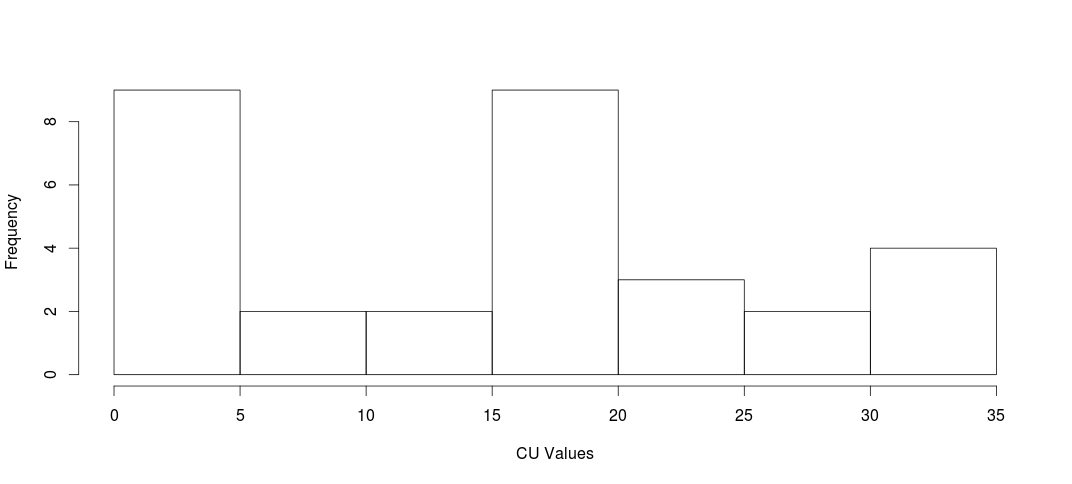
\includegraphics[width=\textwidth]{cu-hist}
                \caption{Hist of CU}
                \label{fig:cu-hist}
        \end{subfigure}%
        ~ %add desired spacing between images, e. g. ~, \quad, \qquad, \hfill etc.
          %(or a blank line to force the subfigure onto a new line)
        \begin{subfigure}[b]{0.45\textwidth}
                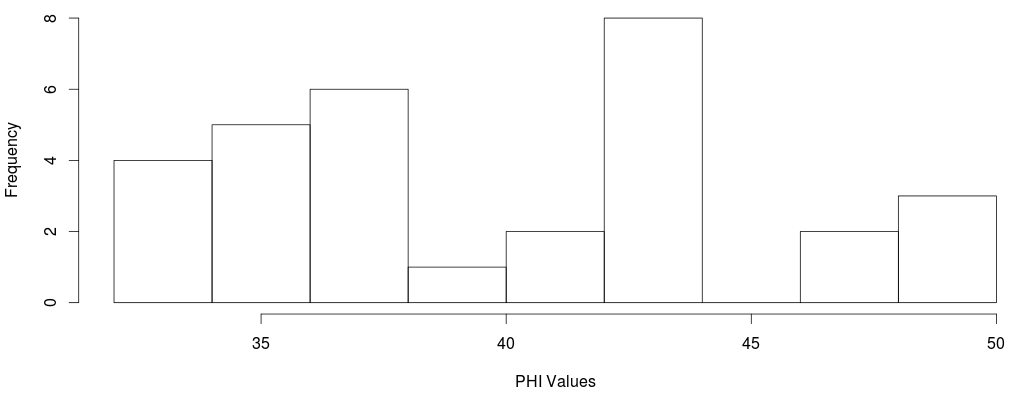
\includegraphics[width=\textwidth]{phi-hist}
                \caption{Hist of PHI}
                \label{fig:phi-hist}
        \end{subfigure}
        ~ %add desired spacing between images, e. g. ~, \quad, \qquad, \hfill etc.
          %(or a blank line to force the subfigure onto a new line)
        \begin{subfigure}[b]{0.45\textwidth}
                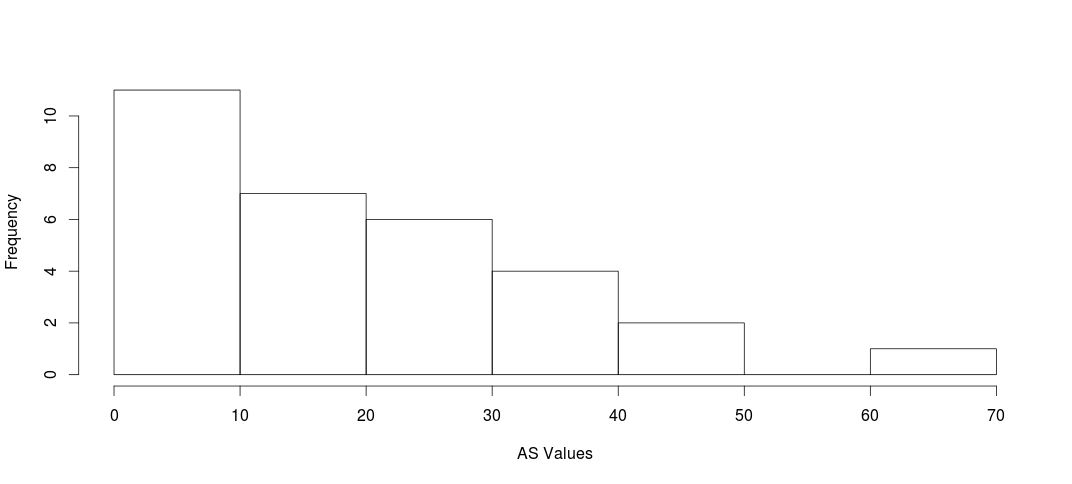
\includegraphics[width=\textwidth]{as-hist}
                \caption{Hist of AS}
                \label{fig:as-hist}
        \end{subfigure}
        ~ %add desired spacing between images, e. g. ~, \quad, \qquad, \hfill etc.
          %(or a blank line to force the subfigure onto a new line)
        \begin{subfigure}[b]{0.45\textwidth}
                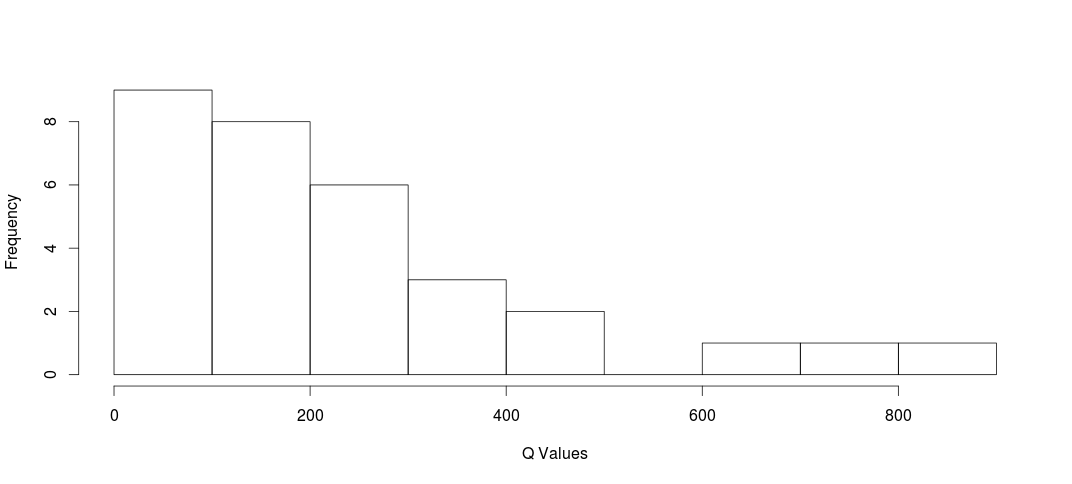
\includegraphics[width=\textwidth]{q-hist}
                \caption{Hist of Q}
                \label{fig:q-hist}
        \end{subfigure}
        \caption{Histograms of the Variables}
        \label{fig:histograms}
\end{figure}



\section{Relationships between the Variables}
We show a scatterplot matrix between all variables in Figure~\ref{fig:pairs}. The top row of this scatterplot matrix gives the scatterplots of Q against each of the other three input variables. Additionally, we show the univariate relationship between our outcome variable Q and the input variables in Table~\ref{table:corr-q}. From this table, we can notice that the correlation between CU and Q and between PHI and Q is significant at the p $<$ 0.05 level.
\begin{figure}[H]
  \centering
  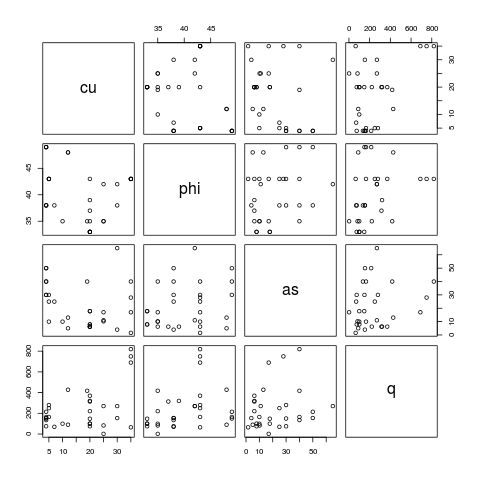
\includegraphics[width=0.5\textwidth]{pairs}
  \caption{Scatterplot of all the variables}
  \label{fig:pairs}
\end{figure}


\begin{table}[H]
\centering

\begin{tabular}{*5c}
\toprule
&  \multicolumn{2}{c}{Correlation (p-value) with Q} \\
\midrule
{}   & Pearson   & Spearman    \\
CU & 0.4595897(0.009293) & 0.1952728(0.2925)   \\
% &  (0.1257239,0.6999433) &    \\
AS   & 0.1964417(0.2895)   & 0.2026105(0.2743)  \\
%  & (-0.1697116,0.5149384)   &   \\
PHI & 0.3082577(0.09158)  & 0.3982587(0.02649)  \\
% & (-0.0517331,0.5973504)  &   \\
\bottomrule
\end{tabular}
\caption{Correlations between the Input Variables and Q}
\label{table:corr-q}
\end{table}

%The 95\% Confidence Interval for Pearson's correlation between CU and Q is (0.1257239,0.6999433)\\
%The 95\% Confidence Interval for Pearson's correlation between AS and Q is (-0.1697116,0.5149384)\\
%The 95\% Confidence Interval for Pearson's correlation between PHI and Q is (-0.0517331,0.5973504)\\
We also provide information about the correlations between our input variables in table~\ref{table:corr}. From this table we can observe that none of the correlations between the input variables is significant at the p $<$ 0.05 level

\begin{table}[htbp]
  \small
  \centering
  \caption{Correlations between Input Variables}
  \subfloat[Pearson Correlation]{%
    \hspace{.5cm}%
    \begin{tabular}{ | l | p{3.9cm} | p{3.9cm} | p{3.9cm} |}
    \hline
     & AS & CU & PHI \\ \hline
    AS & 1 & -0.2596521(0.1584)  & 0.2605386(0.1569)  \\ \hline
    % &  & (-0.5622613,0.1042825) &  (-0.1033419,0.5629112) \\ \hline
    CU & -0.2596521(0.1584)   & 1 & -0.2176558(0.2395) \\ \hline
    % &  (-0.5622613,0.1042825)  &  & (-0.5310399,0.1481069) \\ \hline
    PHI & 0.2605386(0.1569)  & -0.2176558(0.2395) & 1 \\ \hline
    % &  (-0.1033419,0.5629112) & (-0.5310399,0.1481069) &  \\ \hline
    \end{tabular}
    \label{table:corr-p}
    \hspace{.5cm}%
  }\hspace{1cm}
  \subfloat[Spearman Correlation]{%
    \hspace{.5cm}%
    \begin{tabular}{ | l | l | l | l |}
    \hline
     & AS & CU & PHI \\ \hline
    AS & 1 & -0.3944457(0.0281) & 0.204013(0.271) \\ \hline
    CU & -0.3944457(0.0281) & 1 & -0.2161602(0.2428) \\ \hline
    PHI & 0.204013(0.271) & -0.2161602(0.2428) & 1 \\ \hline
    \end{tabular}
    \label{table:corr-sp}
    \hspace{.5cm}%
  }
  \label{table:corr}
\end{table}


\section{Fitting the Models}\label{sec:models}
Let us keep in mind that the ultimate aim of our final model is to determine whether there is an association between VARIABLE(s) and Q. 
Therefore, it would seem reasonable to model CONFOUNDER FIRST and then enter CU into the model and see whether it is associated with Q. We can do this in the opposite way by enetering CU into the model first and then follow it by PHI and AS in turn to see what impact each of them would have on the model.

\subsection{Modelling the Relationship between CU and Q (Model 1)}\label{sec:cumodel}
In this section, we are going to build a simple linear regression model using just CU as input and Q as output. After using R's lm() function, the model looks as follows:\\
\begin{equation}
\label{eq:cu}
Q = 92.890    +    8.557*CU 
\end{equation}       
By examining equation~\ref{eq:cu}, we observe that an increase, or decrease, of CU by one unit, causes an increase, or decrease, in Q by 8.557 units\\

\begin{figure}[H]
  \centering
  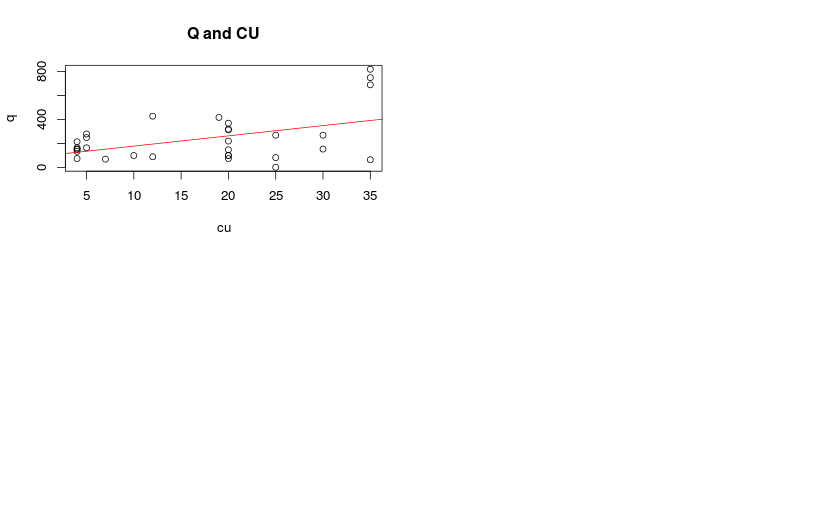
\includegraphics[width=0.6986\textwidth]{cu-line}
  \caption{The Relationship between CU and Q}
  \label{fig:cu-line}
\end{figure}

Now after building the model that describes the relationship between CU and Q, let us plot the input variable CU against the residuals. As Figure~\ref{fig:mod1-resid1} shows, the residual values do not seem to have a particular pattern and they are randomly scattered around zero (as we stated in Section~\ref{sec:residuals}).
\begin{figure}[H]
  \centering
  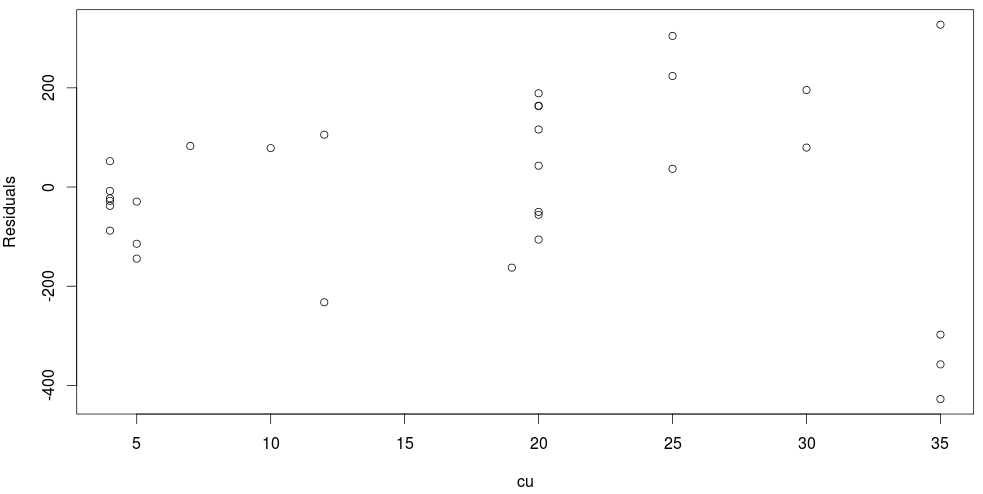
\includegraphics[width=0.6986\textwidth]{mod1-resid1}
  \caption{CU vs Residuals for Model 1}
  \label{fig:mod1-resid1}
\end{figure}

\subsection{Modelling the Relationship between AS and Q (Model 2)} \label{sec:asmodel}
In this section, we are going to build a simple linear regression model using just AS as input and Q as output. After using R's lm() function, the model looks as follows:\\
\begin{equation}
\label{eq:as}
Q = 188.089   +     2.422*AS 
\end{equation}       
By examining equation~\ref{eq:as}, we observe that an increase, or decrease, of AS by one unit, causes an increase, or decrease, in Q by 2.422 units

\begin{figure}[H]
  \centering
  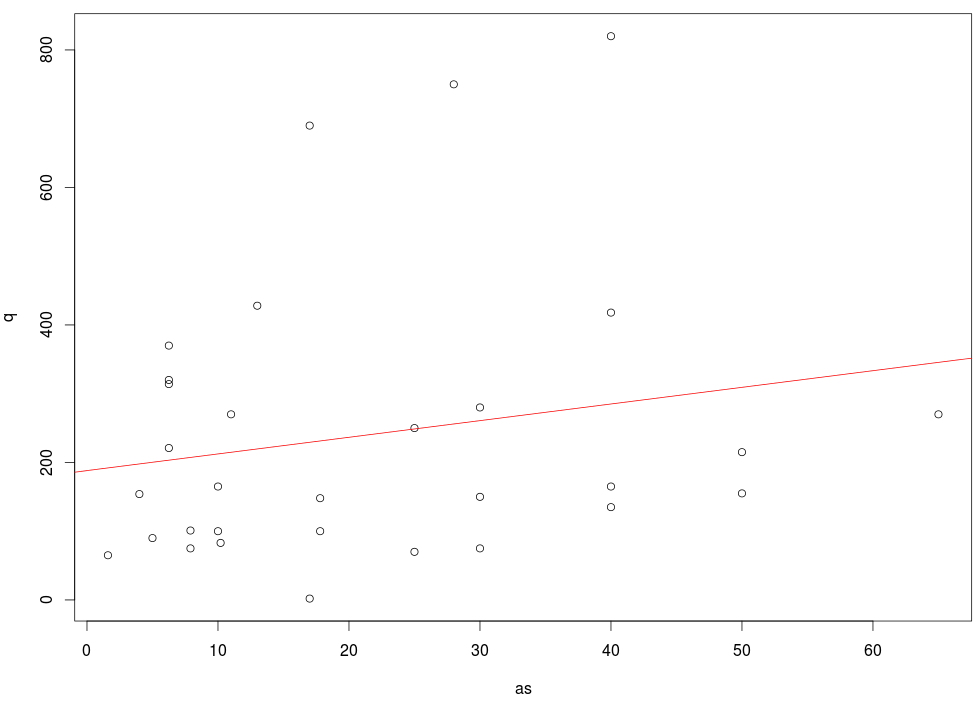
\includegraphics[width=0.6986\textwidth]{as-line}
  \caption{The Relationship between AS and Q}
  \label{fig:as-line}
\end{figure}

Now after building the model that describes the relationship between AS and Q, let us plot the input variable AS against the residuals. As Figure~\ref{fig:mod2-resid1} shows, the residual values do not seem to have a particular pattern and they are randomly scattered around zero (as we stated in Section~\ref{sec:residuals}).

\begin{figure}[H]
  \centering
  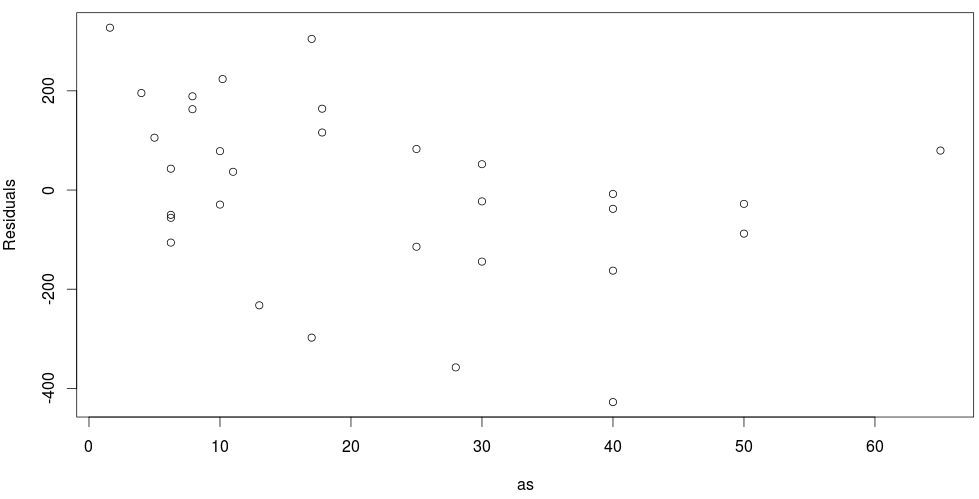
\includegraphics[width=0.6986\textwidth]{mod2-resid1}
  \caption{AS vs Residuals for Model 2}
  \label{fig:mod2-resid1}
\end{figure}

\subsection{Modelling the Relationship between PHI and Q (Model 3)} \label{sec:phimodel}
In this section, we are going to build a simple linear regression model using just PHI as input and Q as output. After using R's lm() function, the model looks as follows:\\
\begin{equation}
\label{eq:phi}
Q =  -244.11    +    12.07*PHI 
\end{equation}       
By examining equation~\ref{eq:phi}, we observe that an increase, or decrease, of PHI by one unit, causes an increase, or decrease, in Q by 12.07 units

\begin{figure}[H]
  \centering
  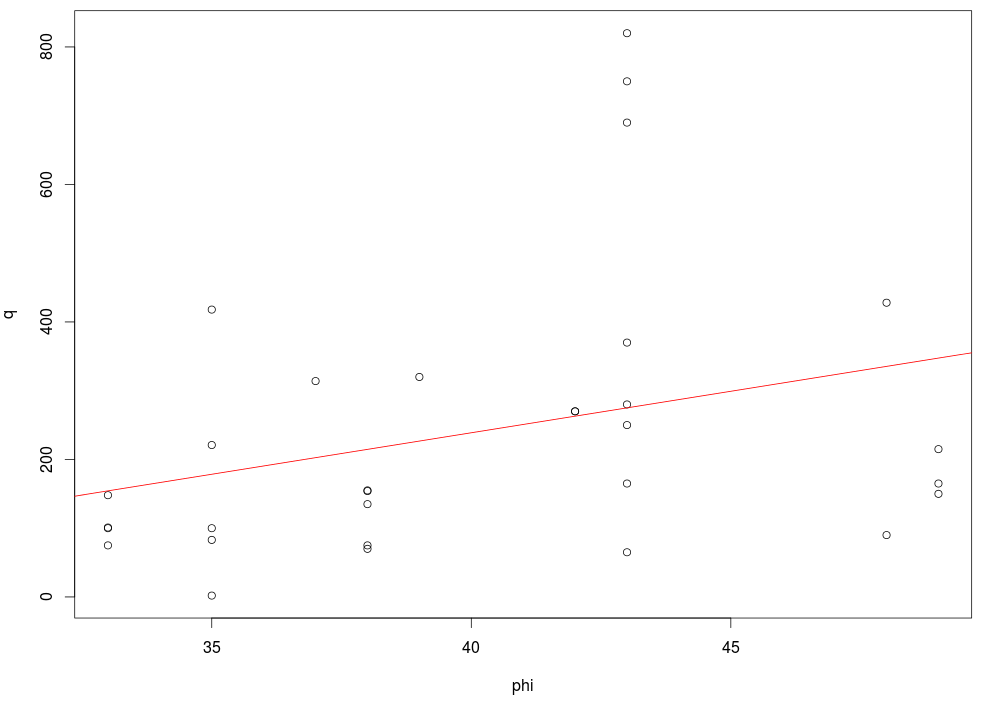
\includegraphics[width=0.6986\textwidth]{phi-line}
  \caption{The Relationship between PHI and Q}
  \label{fig:phi-line}
\end{figure}

Now after building the model that describes the relationship between PHI and Q, let us plot the input variable PHI against the residuals. As Figure~\ref{fig:mod3-resid1} shows, the residual values do not seem to have a particular pattern and they are randomly scattered around zero (as we stated in Section~\ref{sec:residuals}).

\begin{figure}[H]
  \centering
  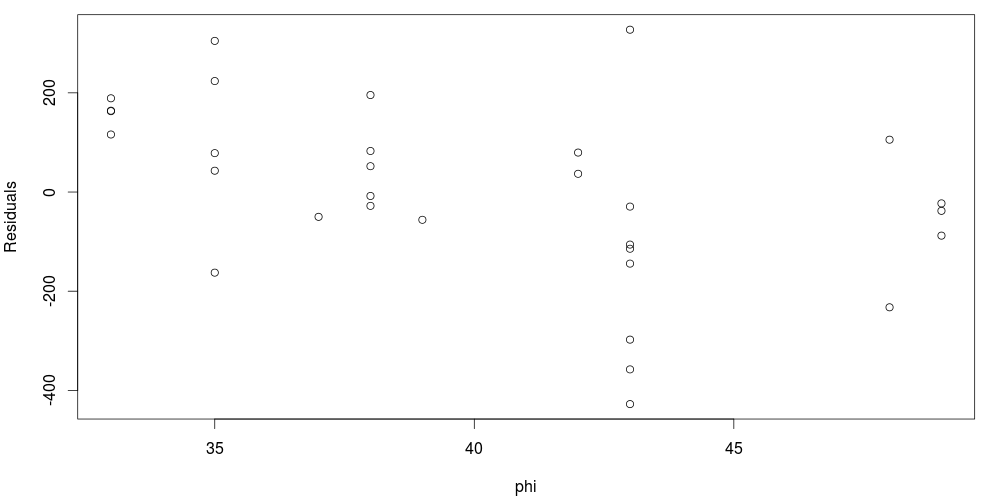
\includegraphics[width=0.6986\textwidth]{mod3-resid1}
  \caption{PHI vs Residuals for Model 3}
  \label{fig:mod3-resid1}
\end{figure}


\subsection{Modelling the Relationship between CU, AS and Q (Model 4)} \label{sec:cuasmodel}
In this section, we are going to build a simple linear regression model using CU and AS as inputs and Q as output. After using R's lm() function, the model looks as follows:\\
\begin{equation}
\label{eq:cuas}
Q = -25.286   +    10.194*CU +       4.174*AS
\end{equation}       
By examining equation~\ref{eq:cuas}, we observe that when fixing AS, an increase, or decrease, of CU by one unit, causes an increase, or decrease, in Q by 10.194 units.
Similarly, when fixing CU, an increase, or decrease, of AS by one unit, causes an increase, or decrease, in Q by 4.174 units.

Now after building the model that describes the relationship between CU, AS and Q, let us plot the input variables CU and AS against the residuals. As Figure~\ref{fig:mod4-resids} shows, the residual values do not seem to have a particular pattern and they are randomly scattered around zero (as we stated in Section~\ref{sec:residuals}).

\begin{figure}[H]
        \centering
        \begin{subfigure}[b]{0.85\textwidth}
                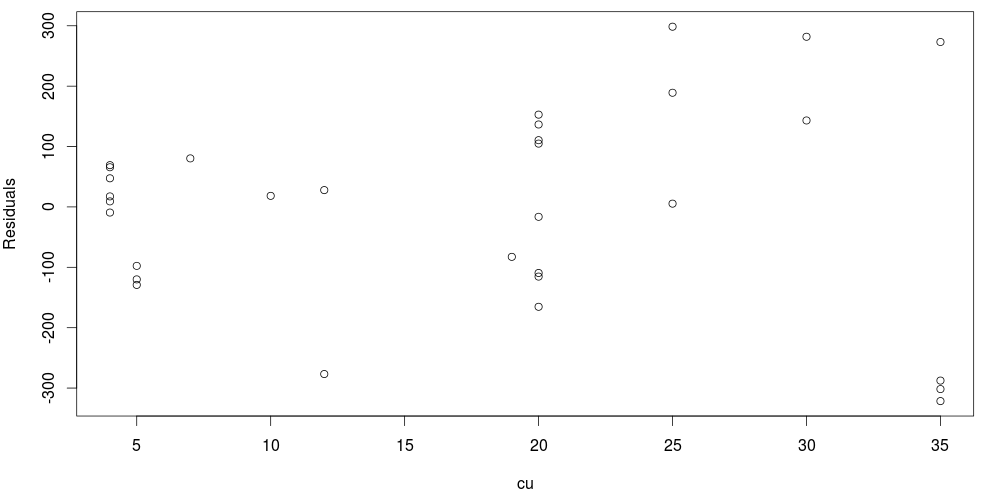
\includegraphics[width=0.986\textwidth]{mod4-resid1}
  		\caption{CU vs Residuals for Model 4}
  		\label{fig:mod4-resid1}
        \end{subfigure}%
        ~ %add desired spacing between images, e. g. ~, \quad, \qquad, \hfill etc.
          %(or a blank line to force the subfigure onto a new line)
        
        \begin{subfigure}[b]{0.85\textwidth}
                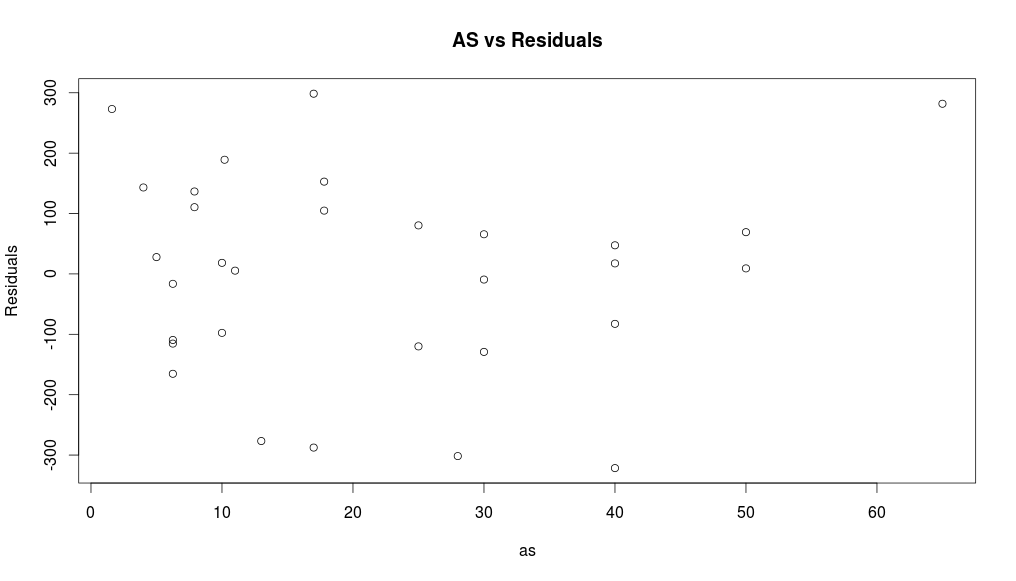
\includegraphics[width=0.96986\textwidth]{mod4-resid2}
  		\caption{AS vs Residuals for Model 4}
 		 \label{fig:mod4-resid2}
        \end{subfigure}
        
        \caption{Input Variables vs Residuals for Model 4}
        \label{fig:mod4-resids}
\end{figure}

\subsection{Modelling the Relationship between CU, PHI and Q (Model 5)} \label{sec:cuphimodel}
In this section, we are going to build a simple linear regression model using CU and PHI as inputs and Q as output. After using R's lm() function, the model looks as follows:\\
\begin{equation}
\label{eq:cuphi}
Q = -610.53  +     10.29*CU   +     16.78*PHI
\end{equation}       
By examining equation~\ref{eq:cuphi}, we observe that when fixing PHI, an increase, or decrease, of CU by one unit, causes an increase, or decrease, in Q by 10.29 units.
Similarly, when fixing CU, an increase, or decrease, of PHI by one unit, causes an increase, or decrease, in Q by 16.78 units.

Now after building the model that describes the relationship between CU, PHI and Q, let us plot the input variables CU and PHI against the residuals. As Figure~\ref{fig:mod5-resids} shows, the residual values do not seem to have a particular pattern and they are randomly scattered around zero (as we stated in Section~\ref{sec:residuals}).

\begin{figure}[H]
        \centering
        \begin{subfigure}[b]{0.85\textwidth}
                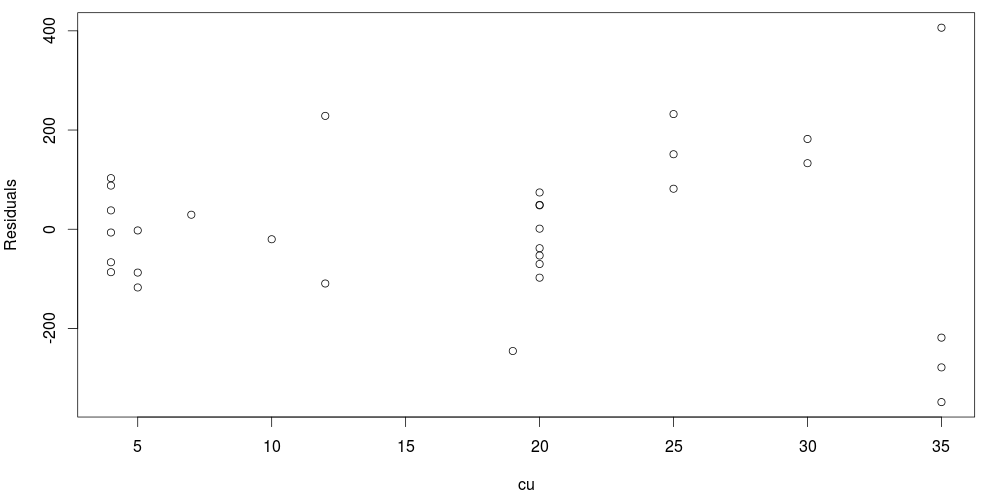
\includegraphics[width=0.96986\textwidth]{mod5-resid1}
  		\caption{CU vs Residuals for Model 5}
  		\label{fig:mod5-resid1}
        \end{subfigure}%
        ~ %add desired spacing between images, e. g. ~, \quad, \qquad, \hfill etc.
          %(or a blank line to force the subfigure onto a new line)
        
        \begin{subfigure}[b]{0.85\textwidth}
                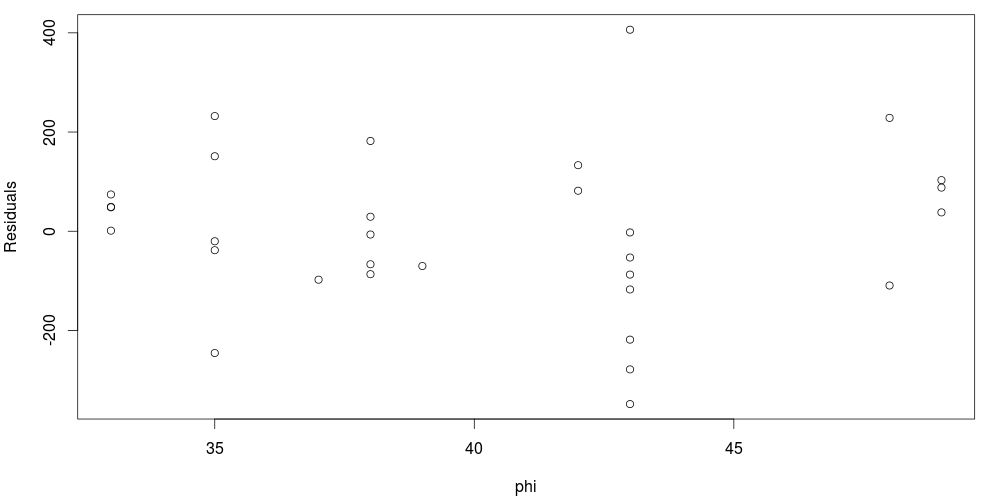
\includegraphics[width=0.96986\textwidth]{mod5-resid2}
 		 \caption{PHI vs Residuals for Model 5}
 		 \label{fig:mod5-resid2}
        \end{subfigure}
        
        \caption{Input Variables vs Residuals for Model 5}
        \label{fig:mod5-resids}
\end{figure}


\subsection{Modelling the Relationship between AS, PHI and Q (Model 6)} \label{sec:asphimodel}
In this section, we are going to build a simple linear regression model using AS and PHI as inputs and Q as output. After using R's lm() function, the model looks as follows:\\
\begin{equation}
\label{eq:asphi}
Q = -226.213  +      1.536*AS   +    10.8*PHI
\end{equation}       
By examining equation~\ref{eq:asphi}, we observe that when fixing PHI, an increase, or decrease, of AS by one unit, causes an increase, or decrease, in Q by 1.536 units.
Similarly, when fixing AS, an increase, or decrease, of PHI by one unit, causes an increase, or decrease, in Q by 10.8 units.

Now after building the model that describes the relationship between AS, PHI and Q, let us plot the input variables AS and PHI against the residuals. As Figure~\ref{fig:mod6-resids} shows, the residual values do not seem to have a particular pattern and they are randomly scattered around zero (as we stated in Section~\ref{sec:residuals}).

\begin{figure}[H]
        \centering
        \begin{subfigure}[b]{0.85\textwidth}
                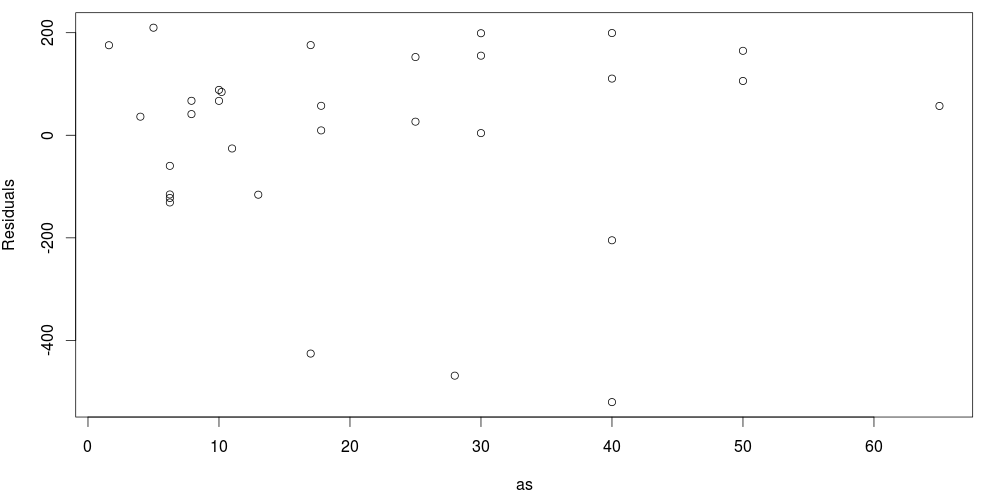
\includegraphics[width=0.96986\textwidth]{mod6-resid1}
   		 \caption{AS vs Residuals for Model 6}
  		\label{fig:mod6-resid1}
        \end{subfigure}%
        ~ %add desired spacing between images, e. g. ~, \quad, \qquad, \hfill etc.
          %(or a blank line to force the subfigure onto a new line)
        
        \begin{subfigure}[b]{0.85\textwidth}
                \centering
  		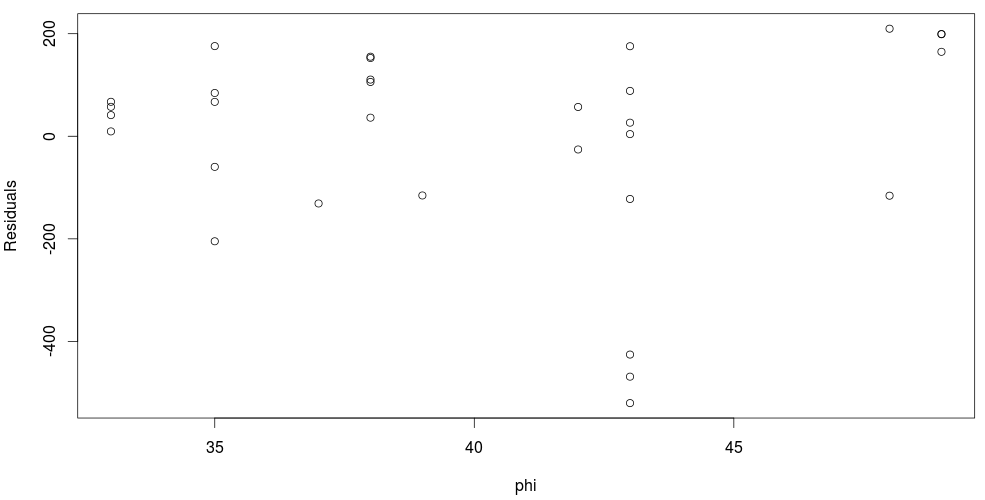
\includegraphics[width=0.96986\textwidth]{mod6-resid2}
  		\caption{PHI vs Residuals for Model 6}
  		\label{fig:mod6-resid2}
        \end{subfigure}
        
        \caption{Input Variables vs Residuals for Model 6}
        \label{fig:mod6-resids}
\end{figure}

\subsection{Modelling the Relationship between CU, AS, PHI and Q (Model 7)} \label{sec:cuasphimodel}
In this section, we are going to build a simple linear regression model using CU, AS and PHI as inputs and Q as output (recall this is the purpose of this study). After using R's lm() function, the model looks as follows:\\
\begin{equation}
\label{eq:cuasphi}
Q = -609.893  +     11.313*CU    +    3.167*AS   +    14.629*PHI
\end{equation}       
By examining equation~\ref{eq:cuasphi}, we observe that when fixing PHI and AS, an increase, or decrease, of CU by one unit, causes an increase, or decrease, in Q by 11.313 units.
Similarly, when fixing CU and AS, an increase, or decrease, of PHI by one unit, causes an increase, or decrease, in Q by 14.629 units. Also, when fixing CU and PHI, an increase, or decrease, of AS by one unit, causes an increase, or decrease, in Q by 3.167 units.

Now after building the model that describes the relationship between CU, AS, PHI and Q, let us plot the input variables CU, AS and PHI against the residuals. As Figure~\ref{fig:mod7-resids} shows, the residual values do not seem to have a particular pattern and they are randomly scattered around zero (as we stated in Section~\ref{sec:residuals}).

\begin{figure}[H]
        \centering
        \begin{subfigure}[b]{0.85\textwidth}
                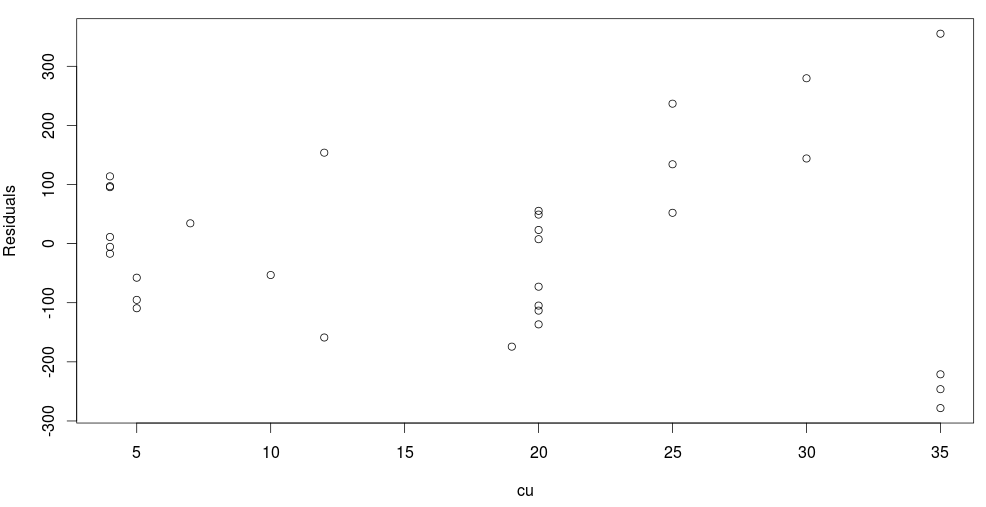
\includegraphics[width=0.96986\textwidth]{mod7-resid1}
  		\caption{CU vs Residuals for Model 7}
  		\label{fig:mod7-resid1}
        \end{subfigure}%
        ~ %add desired spacing between images, e. g. ~, \quad, \qquad, \hfill etc.
          %(or a blank line to force the subfigure onto a new line)
        
        \begin{subfigure}[b]{0.85\textwidth}
                \centering
  		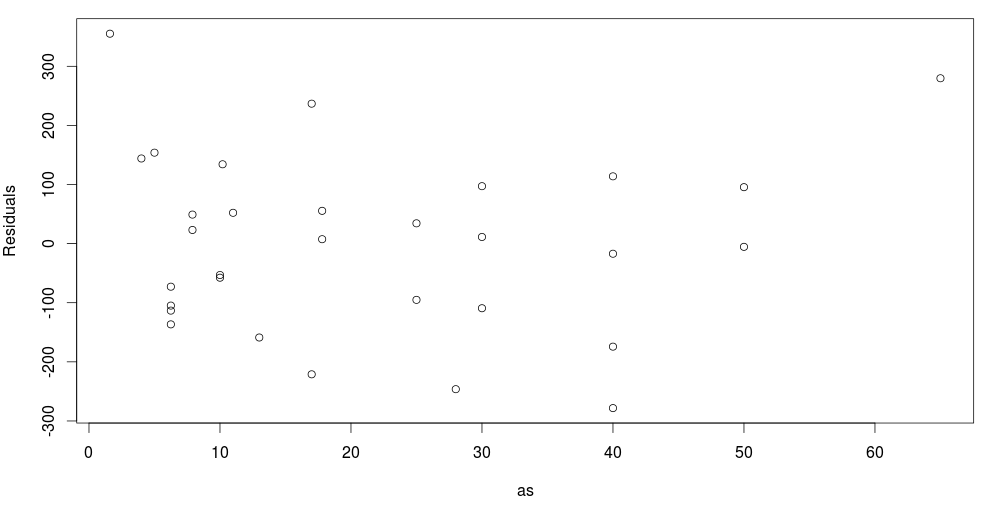
\includegraphics[width=0.96986\textwidth]{mod7-resid2}
  		\caption{AS vs Residuals for Model 7}
  		\label{fig:mod7-resid2}
        \end{subfigure}
        
        \begin{subfigure}[b]{0.85\textwidth}
                \centering
  		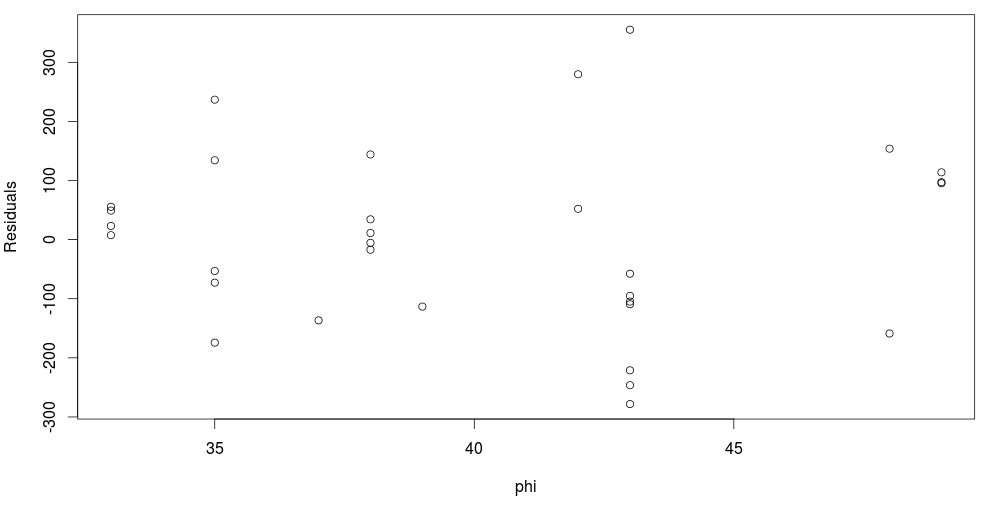
\includegraphics[width=0.96986\textwidth]{mod7-resid3}
  		\caption{PHI vs Residuals for Model 7}
		  \label{fig:mod7-resid3}
        \end{subfigure}
        
        \caption{Input Variables vs Residuals for Model 7}
        \label{fig:mod7-resids}
\end{figure}


\section{Checking the Model Fit}\label{sec:checkmodelfit}
In Section~\ref{sec:examine-fit}, we mentioned five diagnostics that can be used to examine the goodness of fit of a model. Namely, these were: Deviance, BIC, R-Squared, Adjusted R-Squared and the Residuals. We have plotted the individual input variables against the residuals when we built the models in Section~\ref{sec:models}. Table~\ref{table:checkfit} shows the values of the remaining four diagnostics for the seven models.  

%\subsection{Examining Deviance, BIC, R-Squared and Adjusted R-Squared of the Seven models}


\begin{table}[H]
\centering
    \begin{tabular}{ | l | l | l |  l | l |}
    \hline
    Model & Deviance & BIC Value & R-Squared & Adj R-Squared \\ \hline
    Model 1 & 969436 & 419.1411 & 0.2112227 & 0.1840235 \\ \hline
    Model 2 & 1181609 & 425.2766 & 0.03858933 & 0.005437238 \\ \hline
    Model 3 & 1112250 & 423.4013 & 0.09502283 & 0.06381672 \\ \hline
    Model 4 & 838024.3 & 418.0594 &  0.3181453 &  0.2694414 \\ \hline
    Model 5 & 754365.9 & 414.7992 &  0.3862136 &  0.3423717 \\ \hline
    
    Model 6 & 1094468 & 426.3357 &  0.1094908 &  0.04588297 \\ \hline
    Model 7 & 682279.8 &  415.1196 &  0.4448661 &  0.3831845 \\ \hline
    \end{tabular}    
    \caption{Deviance, BIC, R-Squared and Adjusted R-Squared of the Seven models}
    \label{table:checkfit}
\end{table}


As we mentioned in Section~\ref{sec:bic}, a lower BIC indicates a better fitting model. By analysing table~\ref{table:checkfit} we observe that Model 5 has the lowest BIC with Model 7 in second. Howerver, when we examine the value of R-Squared, we realise that Model 7 has the highest R-Squared amongst all the models (see Section~\ref{sec:r2}). This gives us confidence that from amongst the seven models that we created using various combinations of the input variables, Model 7 is the best model that describes the relationship between the input variables CU, AS and PHI and the output variable Q.
%\subsection{Examining Residuals of the Seven models}
%As we stated in Section~\ref{sec:residuals}, the residuals should be randomly scattered around zero when plotted against the input variables.

\bibliographystyle{plain}
\bibliography{report}
\end{document}

